\documentclass[11pt, letterpaper]{article}
\usepackage[utf8]{inputenc}
\usepackage[margin=1in]{geometry}
\usepackage{enumitem}
\usepackage{indentfirst}
\usepackage{titling}
\usepackage{graphicx}
\usepackage{amsmath}
\usepackage{mathtools}
\usepackage{hyperref}
\graphicspath{ {./} }
\DeclareMathAlphabet{\altmathcal}{OMS}{cmsy}{m}{n}

\setlength{\parindent}{0cm}
\setlength{\parskip}{1em}
\renewcommand{\baselinestretch}{1.5}

\hypersetup{
    colorlinks=true,
    linkcolor=cyan,
    filecolor=magenta,      
    urlcolor=blue,
}

\title{Chapter III: Electric Potential}
\author{Chenyi Zhu}
\date{Jan 15th, 2020}

\begin{document}


\begin{titlingpage}
	\maketitle
	
	\begin{figure}[h!]
		\centering
		
\includegraphics[scale=0.6]{emergencies}
		\label{fig:comedian}
	\end{figure}
		
\end{titlingpage}
	
\section{Review: Gravitational Potential and Potential Energy.} 

	We will start reviewing gravitational potential energy first and move on to gravitational potential. 
	Note that the main ideas behind these concepts apply also to electric potential and potential 
	energy, so please do not take this review lightly!
	\subsection{Gravitational Potential Energy}
	We have seen in Chapter I that: \[\vec{F}_g = -G\frac{Mm}{r^2}\, \hat{r}\] where 
	$G = 6.67\times 10^{-11}\,N\cdot m^2/kg^2$, where $\hat{r}$ points radially outward from
	COM. Assuming Earth to be spherical, gravitational field $\vec{g}$ is defined as 
	gravitational force per unit mass, is given by: \[\vec{g} = \frac{\vec{F}_g}{m} = -\frac{GM}{r^2}
	\, \hat{r}\] and note that $\vec{g}$ only depends on $M$, the mass that creates the field, and
	$r$, distance from $M$.
	
	Imagine that we are on a spaceship and trying to move from point $A$ to $B$, under the 
	influence of the gravitational field.
	\begin{figure}[h!]
		\centering
		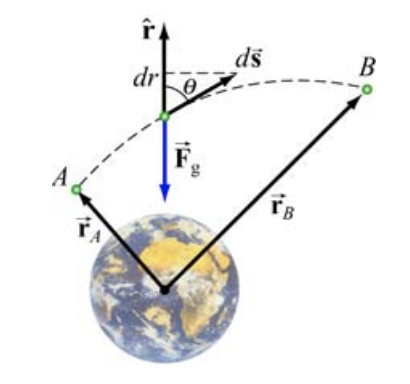
\includegraphics[scale=0.6]{earth}
		\caption{Potential difference.}
		\label{fig:earth}
	\end{figure}
	
	\noindent The work done by gravity to move us (of mass $m$) could be computed by the line
	integral: 
	\begin{equation}\label{eqn:work-1}
		\centering
		\boxed{W_g = \int \vec{F}_g \cdot \, d\vec{s} = \int_{r_A}^{r_B} \left(-\frac{GMm}{r^2}\right) \,
		dr = \frac{GMm}{r}\bigg|_{r_A}^{r_B} = GMm \left( \frac{1}{r_B} - \frac{1}{r_A} \right)}
	\end{equation}
	which confirms what we have already known about work: it is independent of the path taken
	and only depends on the path taken. Think about what happends when you break the non-linear
	path between A and B down into small vectors parallel to the path $d\vec{s}$. Because work is
	done only when the direction of the force applied is parallel to the direction of the path taken, 
	we are able to convert $d\vec{s}$ to $dr$. 
	
	Here is another case: when we are not on the spaceship, but are near the Earth's surface. The 
	gravitational field is pretty much constant, with a magnitude $g=GM/r_E^2 \approx 9.8\, m/s^2$.
	
	\begin{figure}[h!]
		\centering
		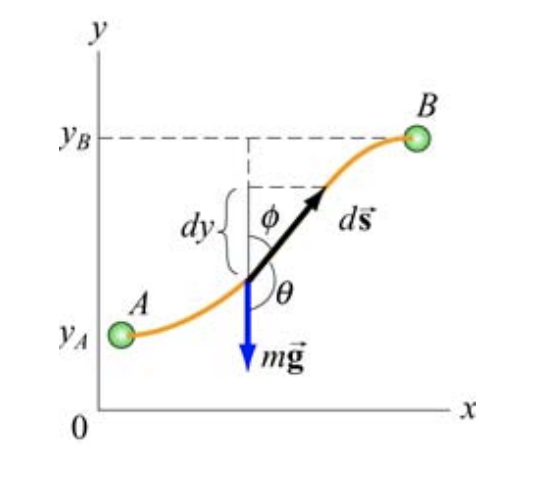
\includegraphics[scale=0.5]{earth_surface}
		\caption{Near Earth's surface.}
	\end{figure}		
	\noindent The work done by gravity moving an object from $A$ to $B$ is given by the following:
	\begin{equation}\label{eqn:work-2}
		\centering
		\boxed{W_g = \int \vec{F}_g\cdot \, d\vec{s} = \int_A^B mg\cos\theta\, ds = -\int_A^B mg\cos
		\phi\, ds = \int_{y_A}^{y_B} mg\, dy = -mg(y_B - y_A)}
	\end{equation}
	\textbf{Note}: In our case, if the line integral is closed curve, then the integral evaluates to $0$;
	no work is done. Thus we say that the gravitational force is a \textbf{conservative} force. More
	generally, we say a force is conservative if its line integral around a closed loop vanishes:
	\begin{equation}\label{eqn:cauchy}
		\boxed{\oint\vec{F}\cdot\, d\vec{s} = 0}
	\end{equation}
	
	We know that work is associated with potential energy. When dealing with a conservative force, 
	it is often convenient to introduce the concept of potential energy $U$:
	\begin{equation}\label{eqn:potential-energy}
		\boxed{\Delta U = U_B - U_A = -\int_A^B \vec{F}\cdot\, d\vec{s} = -W}
	\end{equation}
	where $W$ is the work done \textbf{by} the force \textbf{on} the object. Let us rewrite the
	potential energy: \[U_g = -\frac{GMm}{r} + U_0\] \textbf{Note}: Its relationship with equations (4)
	and (1). I suggest that you try deriving this last expression yourself! I will start you off:
	rearrange $U_g - U_0 = -\frac{GMm}{r} \rightarrow ...$
	
	\subsection{Gravitational Potential}
	Now we are going to derive gravitational potential from $\Delta U$:
	\begin{equation}\label{eqn:potential}
		\boxed{\Delta V_g = \frac{\Delta U_g}{m} = -\int_A^B \frac{\vec{F}_g}{m}\cdot\, d\vec{s} = 
		-\int_A^B \vec{g}\cdot\, d\vec{s}}
	\end{equation}
	where $\Delta V_g$ is the negative work done per unit mass by gravity to move a particle
	from A to B.
	
	\section{Electric Potential and Potential Energy.}
	\subsection{Electric Potential}
	Now, after we have reviewed gravitation, electrostatics is very similar. It has a distance
	dependency of $r^{-2}$,  and the electric force is also a \textbf{conservative} force. We define
	the electric potential difference between two points $A$ and $B$ as:
	\begin{equation}\label{eqn:electric-pot}
		\boxed{\Delta V=-\int_A^B \frac{\vec{F}_e}{q_0}\cdot\, d\vec{s}=-\int_A^B \vec{E}\cdot\, d
		\vec{s}}
	\end{equation}
	where $q_0$ is the infinitesimal test charge. $\Delta V$ represents the work/unit charge to 
	move the test charge from point $A$ to $B$, \textit{without changing its kinetic energy}. The 
	units of electric potential is volt ($1\, V = 1\, J/C$).
	
	\subsection{Electric Potential Energy}
	Please do not confuse the concepts of potential and potential energy! They represent very
	different things. However,, they do have a correlation:
	\begin{equation}\label{eqn:electric-pot-energy}
		\boxed{\Delta U=q_0\Delta V}
	\end{equation}
	
	\newpage	
	\subsection{Electric Potential due to Point Charges}
	Consider point charge $Q$, and the electric field it produces $\vec{E} = (Q/4\pi
	\varepsilon_0r^2)\hat{r}$. 
	\begin{figure}[h!]
		\centering
		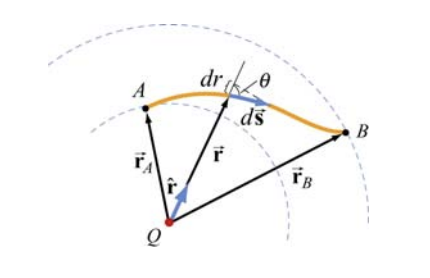
\includegraphics[scale=0.8]{single-charge-pot}
		\caption{Potential difference due to point charge Q.}
	\end{figure}
	
	Apply $\hat{r}\cdot d\vec{s} = ds\cos{\theta} = dr$:
	\begin{equation}\label{eqn:point-chagre-pot}
		\boxed{\Delta V = V_B - V_A = -\int_A^B \frac{Q}{4\pi\varepsilon_0 r^2}\, dr = \frac{Q}{4\pi
		\varepsilon_0}\left(\frac{1}{r_B}-\frac{1}{r_A}\right)}
	\end{equation}
	
	Again, note path independence.
	
	When we discuss the concept of ``potential'' at a given point, it is important that we pick the
	right reference point. Usually, we want the potential at our reference point to be $0$ (standard
	m.o.), which means the reference point will be infinitely far away: \[V_P = -\int_\infty ^P \vec{E}
	\cdot\, d\vec{s}\] and with this reference, our potential simply becomes:
	\begin{equation}
		\boxed{V(r) = \frac{1}{4\pi\varepsilon}\frac{Q}{r}}
	\end{equation}
	\textbf{Note}: This is a scalar quantity and does not specify direction. This means applying 
	superposition principle has never been easier. Now just add up the potential due to each 
	point charges without worrying about vectors.
	\newpage
	\subsection{Continuous Charge Distribution}
	\begin{figure}[h!]
		\centering
		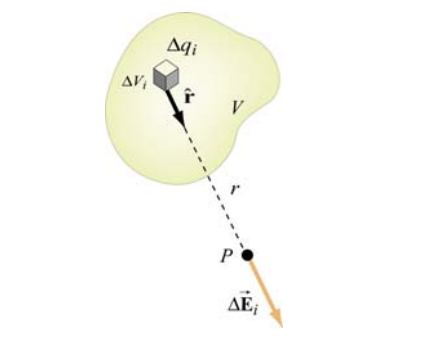
\includegraphics[scale=0.6]{volume}
		\caption{Continuous charge distribution due to bean.}
	\end{figure}
	Consider a solid charged bean. The potential at point P can be found by summing over all 
	individual infinitesimal charges $dq$:
	\begin{equation}
		dV = \frac{1}{4\pi\varepsilon}\frac{dq}{r} \Rightarrow \boxed{V = \frac{1}{4\pi\varepsilon}\int
		\frac{dq}{r}}
	\end{equation}
	
	\subsection{Deriving the Electric Field from Potential}
	A simpler but rigorous definition of electric potential is: consider two points separated by a 
	small distance $d\vec{s}$, we will obtain the following differential: $\Delta V = -\vec{E}\cdot\,
	d\vec{s}$, and in Cartesian coordinates we have: $\vec{E} = E_x\hat{i} + E_y\hat{j} + E_z\hat{k}$
	and $d\vec{s} = dx\hat{i} + dy\hat{j} + dz\hat{k} \implies \vec{E} = E_xdx + E_ydy + E_zdz$, and:
	\begin{equation}
		\boxed{E_x = -\frac{\partial V}{\partial x}, E_y = -\frac{\partial V}{\partial y}, E_z = -\frac{\partial
		V}{\partial z}}
	\end{equation}
	
	using the gradient (``del'') operator.
	If our charge distribution has a spherical symmetry, then the resulting electric field can be a 
	function of the radial distance r, and:
	\begin{equation}
		\boxed{\vec{E} = E_r\hat{r} = -\left(\frac{dV}{dr}\right)\,\hat{r} }
	\end{equation}
	
	\newpage
	
	\subsection{Gradient and Equipotentials}
	We have all seen contour maps in one way or another. Here is an example of its usage in 
	geography as topographic map:
	\begin{figure}[h!]
		\centering 
		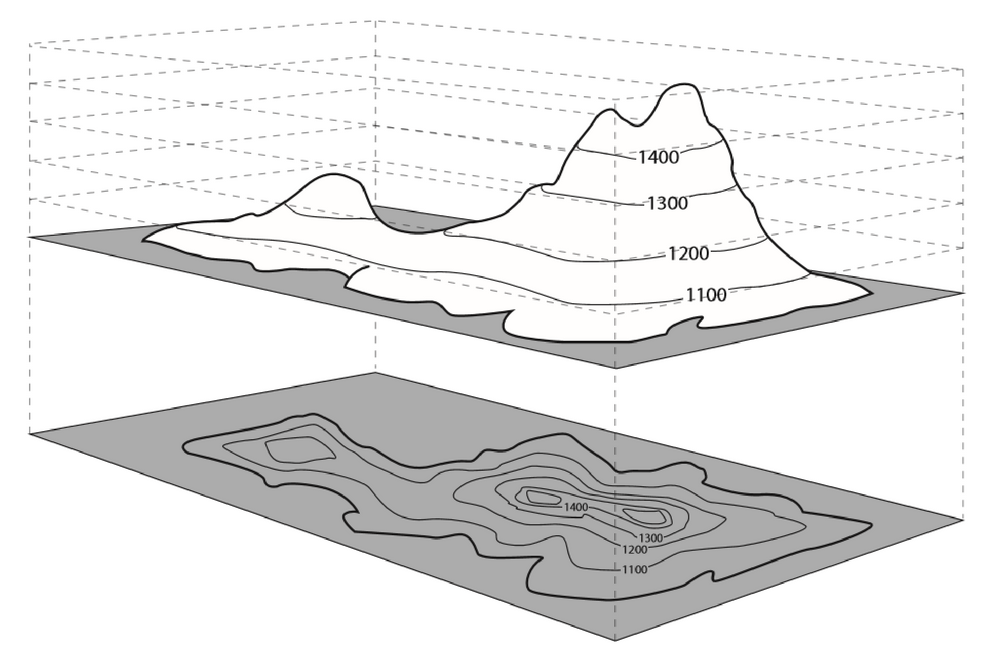
\includegraphics[scale=0.15]{contour}
		\caption{Dissecting a mountain.}
	\end{figure}
	
	Given the contour map in 2D, we can say several things about the structure of the mountain
	in 3D, e.g. where the peaks are, steepness of the mountain, etc. We can do the same with 
	electricity, illustrated by the blue dotted lines in the figure below:
	\begin{figure}[h!]
		\centering
		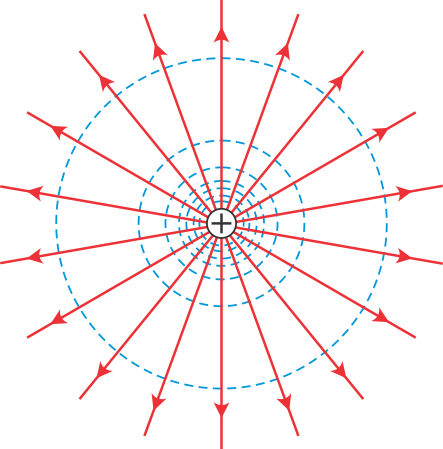
\includegraphics[scale=1.7]{equipotent}
		\caption{Equipotential surface of a single positive point charge.}
	\end{figure}
	
	Here are the general properties of equipotential surfaces:
	\begin{itemize}
		\item The electric field lines are perpendicular to the equipotentials and point from higher
		to lower potentials.
		\item By symmetry, the equipotential surfaces produced by the a point charge form a family
		of concentric spheres, and for a constant electric field, a family of planes perpendicular to 
		the field lines.
		\item The tangential component of the electric field along the equipotential surface is 0, o/w
		non-vanishing work would be done to move the charge along the surface.
		\item No work is required to move particles along one equipotential surface.
	\end{itemize}

\section{Exercises.}
\subsection{Warm-up}

	\textbf{Problem 1}: Recall the chart given to you in Chapter 2, and some homework problems 
	you have seen. Now, instead of finding the electric field at a given point P, I will ask you to find
	the electric potential at $P$, all the conditions remain the same.
	\begin{itemize}
		\item Uniformly charged line, both finite and infinite.
		\item Uniformly charged ring.
		\item Uniformly charged disk.
	\end{itemize}
	
\subsection{More Practice}
	%3.32
	\textbf{Problem 2}: Find the electric field potential and strength at the center of a hemisphere
	of radius $R$ with uniform surface charge density $\sigma$.
	
	%3.36
	\textbf{Problem 3}: Determine the electric field strength vector if the potential of this field 
	depends on $x$, $y$ coordinates as: a) $\varphi = a(x^2+y^2)$; and b) $\varphi = axy$ where
	$a$ is a constant. Draw the approximate shapes of these fields using lines of force (in the $x$,
	$y$ plane).
	
	%3.38
	\textbf{Problem 4}: A charge $q$ is uniformly distributed over the volume of a sphere of 
	radius $R$. Assuming permittivity to be equal to unity throughout, find the potential
	\begin{itemize}
		\item at the center of the sphere;
		\item inside the sphere as a function of the distance $r$ from its center.
	\end{itemize}
		
	\pagebreak
	%3.42
	\textbf{Problem 5}: Two thin parallel threads carry a uniform charge with linear charge 
	densities $\lambda$ and $-\lambda$, separated by a distance $l$. Find the potential of
	the electric field and its magnitude at the distance $r \gg l$ at the angle $\theta$ to the 
	vector $\vec{l}$.
	\begin{figure}[h!]
		\centering
		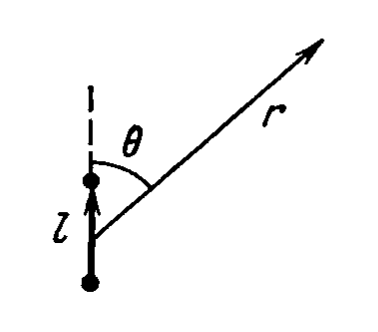
\includegraphics[scale=0.5]{two-lines}
		\caption{Two parallel lines.}
	\end{figure}
	
	\textbf{Problem 6}: Two coaxial rings, each of radius $R$, made of thin wire are separated
	by a small distance $l$ $(l \ll R)$ and carry the charges $q$ and $-q$. Find the electric 
	field magnitude and potential at the axis of the system as a function of the $x$ coordinate.  
	Plot the functions and observe what happens when $|x| \gg R$. 

	%3.50
	\textbf{Problem 7}: Determine the potential $\varphi(x,y,z)$ of an electrostatic field 
	$\vec{E} = ay\hat{i} +(ax+bz)\hat{j} + by\hat{k}$, where $a$ and $b$ are constants
	and $\hat{i}$, $\hat{j}$, and $\hat{k}$ are unit vectors in Cartesian coordinates.
	
		
	
	
		

\end{document}
